\documentclass[11pt,letterpaper]{article}
\usepackage[margin=0.88in]{geometry}
\usepackage[T1]{fontenc}
\usepackage{lmodern}
\usepackage{amsmath,amssymb,amsthm,mathtools}
\usepackage{booktabs,array,longtable,tabularx}
\usepackage{tikz}
\usetikzlibrary{arrows.meta,positioning,shapes.geometric,calc}
\usepackage[hidelinks]{hyperref}
\usepackage{microtype}
\usepackage{enumitem}
\usepackage{fancyhdr}
\usepackage{caption}
\usepackage{xcolor}
\hypersetup{pdftitle={FDWC research manuscript},pdfauthor={Brian Tenneson (research direction); AI-assisted manuscript}}
\setlength{\parskip}{0.30em}
\setlength{\parindent}{0pt}
\setlength{\headheight}{14pt}
\setlist[itemize]{leftmargin=1.5em,itemsep=0.15em}
\newtheorem{theorem}{Theorem}[section]
\newtheorem{proposition}[theorem]{Proposition}
\newtheorem{lemma}[theorem]{Lemma}
\newtheorem{corollary}[theorem]{Corollary}
\theoremstyle{definition}
\newtheorem{definition}[theorem]{Definition}
\newtheorem{example}[theorem]{Example}
\theoremstyle{remark}
\newtheorem{remark}[theorem]{Remark}
\newcommand{\N}{\mathbb{N}}
\newcommand{\Pow}{\mathcal P}
\newcommand{\ck}{\mathsf{Check}}
\newcommand{\Win}{\mathsf{Win}}
\newcommand{\Inf}{+\infty}
\newcommand{\backproof}[1]{\hfill\hyperlink{proof:#1}{\footnotesize Go to proof}}
\newcommand{\backstatement}[1]{\hyperlink{stmt:#1}{\footnotesize Return to statement}}
\pagestyle{fancy}
\fancyhf{}
\fancyhead[L]{\footnotesize FDWC certified mathematical research}
\fancyhead[R]{\footnotesize \leveltag}
\fancyfoot[L]{\footnotesize Research direction: Brian Tenneson}
\fancyfoot[R]{\footnotesize \thepage}
\newcommand{\smalltag}[1]{\textsf{\footnotesize #1}}
\begin{document}
\newcommand{\leveltag}{W1}
\title{\bfseries\LARGE Certified Revision as a Costed Mathematical Game\\[0.45em]\large Multiarticle synthesis of conservative compilation, successor evidence, and forced settlement}
\author{Brian Tenneson\\\normalsize Research direction; AI-assisted mathematical drafting}
\date{17 November 2026 --- FDWC W1 manuscript}
\maketitle
\begin{center}\small See the AI disclaimer that follows this essay.\end{center}
\begin{abstract}A conservative rule extension, an accepted revision, an economical revision, and a forced transition to a desirable architecture are different mathematical claims. This Level-1 multiarticle synthesizes two internally developed completions of W0: proof-carrying successor compilation and costed adversarial revision games. It retains W0's finite-cache and finite-game results, makes the certificate gate explicit in a common state model, and proves a new cross-branch result: a finite quotient preserving target, owner, and exact costed successor signatures preserves minimum forced settlement cost. An exact two-token coordination example shows why proof preservation does not by itself establish economic improvement or adversarial force. The paper gives proofs, counterexamples, a verification ledger, and precise boundaries on its finite-model claims.\end{abstract}
\noindent\textbf{Keywords.} certified revision; mathematical games; cost-preserving quotients; proof certificates; basin escape
\tableofcontents
\newpage

\section{The mathematical question}
A provable theorem and an economical way to find or deploy its proof are not the same object. In W0, Part II shows that adding genuinely derived inference rules preserves the base consequence relation; Part III makes revisions dependent on typed, verifier-accepted evidence; Parts IV--V study reachable improvement basins and complete costs; Part VI distinguishes promising paths from adversarially forced outcomes. The present synthesis asks:

\emph{Can a smaller representation of a certified revision process preserve the difference between a possible, economically beneficial revision and one that can actually be forced?}

We pursue two mathematical completions in the analysis: a \emph{certificate branch} (safe derivation and implementation contracts) and a \emph{planning branch} (fully charged revision paths and adversarial choices). The final text is their integrated mathematical theory, not a concatenation of alternative manuscripts.

\begin{figure}[ht]
\centering
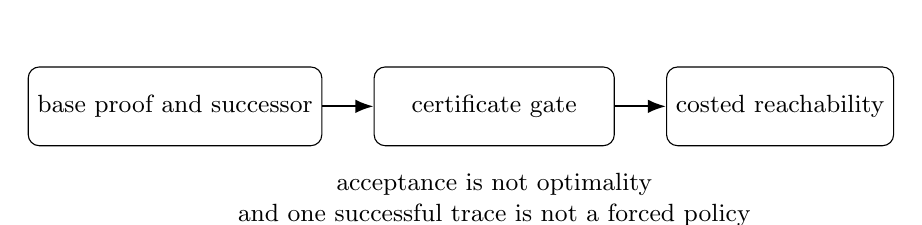
\begin{tikzpicture}[>=Latex, node distance=0.5cm, every node/.style={font=\small}]
\node[draw,rounded corners,minimum width=3.1cm,minimum height=1cm] (a) {base proof and successor};
\node[draw,rounded corners,right=0.65cm of a,minimum width=3.05cm,minimum height=1cm] (b) {certificate gate};
\node[draw,rounded corners,right=0.65cm of b,minimum width=2.85cm,minimum height=1cm] (c) {costed reachability};
\draw[->,thick] (a)--(b);\draw[->,thick] (b)--(c);
\node[below=0.22cm of b,align=center] {acceptance is not optimality\\and one successful trace is not a forced policy};
\end{tikzpicture}
\caption{The two completions meet at a typed, costed transition relation.}
\end{figure}

\section{The proof-carrying branch}
\begin{definition}[Base calculus and certified macro]
Fix a finitary calculus $F$ with a derivability relation $\Gamma\vdash_F\varphi$. A macro $d$ is \emph{certified derived} when each authorized application of $d$ carries a finite derivation in $F$ from precisely the premises used by the application. A \emph{conservative revision} adds such macros without deleting any base rule or changing hypotheses.
\end{definition}

\begin{theorem}[Conservative admissible compilation; inherited, W0 II.2.2 and III.4.4]\label{thm:cons}\hypertarget{stmt:cons}{}
For any $\Gamma$ and any collection $D$ of certified derived rules, $\mathrm{Con}_{F+D}(\Gamma)=\mathrm{Con}_F(\Gamma)$.
\end{theorem}\backproof{cons}

This preserves \emph{which} formulas can be proved. It says nothing about the finite cost of finding them or preserving implementation-specific timing. For example, the calculus $a\to b\to c\to d$ permits a compiled macro $a\Rightarrow d$: proof depth changes while theoremhood does not. W0 III.5 establishes a fully charged benefit only after finite setup costs are included and the repeated workload is sufficiently large.

\begin{definition}[Frozen contract and acceptance]
A finite revision contract contains the following frozen data:\[K=(F,\Gamma,W,I,E,R,O,\kappa,B,Q,V).\] These designate calculus, hypotheses, workload, information rights, environment, simulation obligation, observations, charge model, budget, permissions, and verifier. A proposed edge $x\xrightarrow{c}y$ is \emph{accepted} only after all $K$-mandatory certificates for its update and charge $c$ pass $V$. The edge is not present in the admitted game when a mandatory checker outcome is missing or rejected.
\end{definition}

A ledger record includes old/new code identifiers, the assumptions, proof object, verifier version and outcome, action rights, cost witness, and resulting state. This follows W0 III.4.5 and V.1; a proposed certificate is neither its successful verification nor its actual installation.

\begin{proposition}[Pathwise theoremhood invariant; derived]\label{prop:path}\hypertarget{stmt:path}{}
Suppose all accepted edges install only conservative macros and never change the base hypotheses. Every finite path of accepted revisions has the same $F$-consequence relation at its final architecture as at its initial architecture.
\end{proposition}\backproof{path}

\section{The planning branch: forcing is not possibility}
\begin{definition}[Finite costed revision game]
Let $G=(X_\exists,X_\forall,E,T,c)$ be a finite directed game. $X=X_\exists\sqcup X_\forall$, each nonterminal has a nonempty finite successor set, $T\subseteq X$ is absorbing and denotes a fully certified objective, and $c:E\to\N$ charges the entire admitted transition. At a controller state $X_\exists$ the controller chooses an edge; at an adversary state $X_\forall$ its opponent chooses. An infinite play that never reaches $T$ has cost $+\infty$. Define
\[
  V_G(x)=\inf_{\sigma}\sup_{\tau}\,\mathrm{Cost}_{T}(\mathrm{play}(x,\sigma,\tau)).
\]
A cost is \emph{forced} if one controller strategy bounds it against all legal opponent continuations. There is no hidden fairness or scheduler assumption unless fixed in $K$.
\end{definition}

\begin{theorem}[Finite forced-cost decision; inherited, W0 VI.5.2]\label{thm:finite}\hypertarget{stmt:finite}{}
If $G$ is explicitly represented and all costs are finite nonnegative integers, $V_G(x)$ is either a computable finite nonnegative integer or $+\infty$. A winning strategy and its finite budget can be extracted in the former case; an adversarial avoidance policy can be exhibited in the latter.
\end{theorem}\backproof{finite}

\begin{remark}
The infinite value here means that \emph{this finite complete game's} controller cannot force the target under the frozen turn ownership and legal transitions. It does not establish an impossibility for an unrestricted machine, an incomplete abstraction, or a different scheduler. If a mandatory certificate has not yet been searched for exhaustively, the appropriate external status is unresolved, not $+\infty$.
\end{remark}

\section{A genuine cross-branch surplus: costed quotient invariance}
The proof branch tells us which revisions may be admitted. The planning branch tells us which accepted outcomes can be forced. It is tempting to retain only a final cost or current proof status in a compressed state. Such a quotient need not preserve future actions. The following theorem supplies a sufficient, finite, checkable criterion.

\begin{definition}[Exact costed game congruence]
For an equivalence relation $\sim$ on $X$, write $[x]$ for an equivalence class. Call $\sim$ an \emph{exact costed game congruence} if, whenever $x\sim x'$:
\begin{enumerate}[label=(\roman*)]
\item $x$ and $x'$ have the same turn owner, target status, and all $K$-required local checker/authorization labels;
\item the sets of costed successor classes agree:
\[
\big\{(c(x,y),[y]):x\to y\big\}
=\big\{(c(x',y'),[y']):x'\to y'\big\}.
\]
\end{enumerate}
The quotient game $G/{\sim}$ has classes as states and the displayed pairs as its edges, with their cost and owner labels.
\end{definition}

\begin{theorem}[Exact forcing survives a certified quotient; cross-source surplus]\label{thm:quot}\hypertarget{stmt:quot}{}
For a finite costed game $G$ and an exact costed game congruence $\sim$, each state $x$ has precisely the same minimum forced settlement cost as its quotient class:
\[
\boxed{V_G(x)=V_{G/\sim}([x]).}
\]
Moreover, a winning quotient policy can be lifted to a winning original-state policy with the same forced-cost bound, and a quotient losing-region certificate lifts to the original game.
\end{theorem}\backproof{quot}

\begin{figure}[ht]
\centering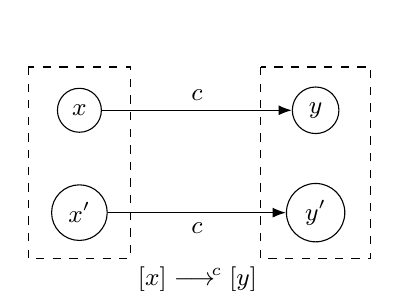
\begin{tikzpicture}[>=Latex, every node/.style={font=\small}]
\node[draw,circle] (a) at (0,0.5) {$x$};\node[draw,circle] (b) at (0,-0.8) {$x'$};
\node[draw,circle] (c) at (3,0.5) {$y$};\node[draw,circle] (d) at (3,-0.8) {$y'$};
\draw[->] (a)--node[above]{$c$}(c);\draw[->] (b)--node[below]{$c$}(d);
\draw[dashed] (-0.65,1.05) rectangle (0.65,-1.38);
\draw[dashed] (2.3,1.05) rectangle (3.7,-1.38);
\node at (1.5,-1.65) {$[x]\longrightarrow^{\!c}[y]$};
\end{tikzpicture}
\caption{Local matching of all costed successor classes permits exact game compression.}
\end{figure}

The hypothesis is deliberately stronger than preserving a terminal score: it preserves \emph{all} legal alternatives and costs. Distinct proof objects may still be kept outside the control-state quotient in an immutable provenance archive, as long as their checker-relevant effects have been captured in the class labels and future transitions.

\begin{corollary}[Certified reduced planning; cross-source surplus]\label{cor:gate}\hypertarget{stmt:gate}{}
If an admitted revision graph uses the W0-style certificate gate and its quotient relation also preserves all gate-relevant labels and legal costed successors, optimal forced cost may be calculated on the quotient and used for the original architecture without changing the mathematical force claim.
\end{corollary}\backproof{gate}

\section{Economy can reverse the apparent order}
\begin{proposition}[Exact workload break-even rule; inherited inequality specialized]\label{prop:break}\hypertarget{stmt:break}{}
For a frozen workload of $N\in\N$ identical episodes, an old execution cost $p$, a new cost $q<p$, and a complete nonnegative acquisition charge $B$, the change is strictly cheaper exactly when $N(p-q)>B$. For integral $N\ge1$, the first profitable episode count is $\lfloor B/(p-q)\rfloor+1$.
\end{proposition}\backproof{break}

\begin{example}[Coordinated basin, inherited W0 IV.13 and V.3]
Let the recurring cost of architectures $A_0,A_u,A_v,A_{uv}$ be $10,11,11,4$. Under the specified finite model, acquiring a joint certificate costs $2$ and installation costs $3$. From the no-evidence state the package is affordable only when the allowed initial budget is at least $5$. With $N=10$ future episodes, the already certified joint route charges $2+3+4N=45$ instead of $10N=100$. But a policy testing one improvement at a time can stop at $A_0$, even though the joint route is beneficial. The transitions are model assumptions, not measured performance.
\end{example}

\begin{figure}[ht]
\centering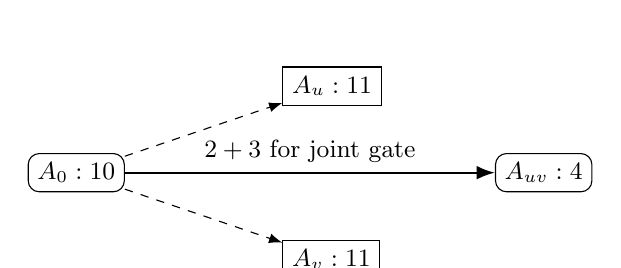
\begin{tikzpicture}[>=Latex, every node/.style={font=\small},node distance=1.6cm]
\node[draw,rounded corners] (o) {$A_0:10$};
\node[draw,above right=0.6cm and 2cm of o] (u) {$A_u:11$};
\node[draw,below right=0.6cm and 2cm of o] (v) {$A_v:11$};
\node[draw,right=4.7cm of o,rounded corners] (uv) {$A_{uv}:4$};
\draw[->,dashed] (o)--(u);\draw[->,dashed](o)--(v);
\draw[->,thick](o)--node[above]{$2+3$ for joint gate}(uv);
\end{tikzpicture}
\caption{A locally stationary single-token policy need not be globally economical.}
\end{figure}

\section{What the synthesis can and cannot settle}
Three counterexamples set the boundary. First, a conservative macro can shorten inference depth while increasing runtime after indexing and checking charges (W0 II.2.5). Second, a path to $T$ may exist but an adversary may select a costed self-loop indefinitely, so possibility is not forcing. Third, states with the same final observed price may have distinct legal successor sets; identifying them without the signature condition can manufacture a false winning strategy.

The verified finite-object result is: given a \emph{complete} explicit accepted revision graph and a checkable stable costed quotient, one may compute its exact forced value on the quotient. The unresolved frontier is how to construct such a faithful finite graph and sufficient summary from an evolving open-ended ATP with partial information or unbounded evidence. That frontier motivates W2.

\section{Research and provenance ledger}
\small
\begin{longtable}{p{0.17\linewidth}p{0.36\linewidth}p{0.35\linewidth}}
\toprule Status & Result & Source and limits \\\midrule\endhead
Inherited & Conservative compilation, finite update stabilization, finite forced-cost game & W0 II.1--II.2, III.4, III.9, VI.5; paper-level source proofs \\
Repaired & Explicit overflow sink for any over-budget game edge & Makes W0 VI.5.2 budget-game proof convention safe at adversarial vertices \\
Derived & Pathwise theoremhood invariant & Induction from W0's conservative gate \\
Cross-source surplus & Theorem~\ref{thm:quot}: quotient preserves adversarial minimum cost & Combines W0 certificate/ledger semantics (III,V) with W0 costed games (VI), using a new matching-signature proof \\
Derived & Corollary~\ref{cor:gate}, certificate-gated quotient use & Requires an explicitly complete finite game; not a general compiler \\
Inherited /\newline specialized & Break-even arithmetic and two-token example & W0 IV.13, V.3, V.6 \\
Unresolved & Building a faithful finite state/edge abstraction from arbitrary ATP behavior & W0 V.7 and VI.10 \\
\bottomrule
\end{longtable}
\normalsize


\section{Bounded six-level consequence exploration}
The Multiarticle procedure also requests low-in-fan consequence mining. Here is one \emph{bounded, explicit} six-level dependency chain; it is not claimed to be an exhaustive closure of either W0 or its two internal completions.
\begin{enumerate}[label=+\arabic*.]
\item Every accepted new macro has a base derivation (certificate branch, W0 II--III).
\item Every finite path of such admitted macros preserves base consequence sets (Proposition~\ref{prop:path}).
\item Such accepted paths can be encoded as a finite costed game when all state/permission coordinates are explicit (planning branch, W0 V--VI).
\item Exact forced reachability in this game is decided by a finite attractor and a budget expansion (Theorem~\ref{thm:finite}).
\item A relation matching owners, targets, gate labels and charged successor classes preserves each budget-attractor stage (Theorem~\ref{thm:quot}).
\item Therefore one can lift a quotient winning policy and its cost certificate into the original admitted revision model (Corollary~\ref{cor:gate}).
\end{enumerate}
The sixth statement is the selected cross-branch surplus: neither merely listing proof-preservation lemmas nor merely listing shortest-path values establishes the typed quotient transfer. Its validity is restricted to the exact game congruence hypothesis; weaker retrospective compression is not silently substituted.

\section{Comparison and audit of internal Level-1 developments}
The proof-carrying completion supplied a strong theoremhood invariant and exact gate obligations, but no adversarial policy. The costed-game completion supplied forcing and full-charge metrics, but could have treated a proposed update as a legal edge without the gate. The synthesis installs the gate \emph{before} game construction and asks for a quotient certificate \emph{after} the state is made contract-complete. This adds a cross-source logical guarantee; it does not dominate either branch on all metrics. The mathematical limitation is the need for a fully represented finite state graph. The first audit restricted all force claims to that finite graph, kept economic comparison separate, and preserved W0's original experiments as historical reports only.

\section{PROOFS}
\hypertarget{proof:cons}{}\subsection*{Theorem \ref{thm:cons}: conservative compilation} \backstatement{cons}
Every $F$-proof remains a proof in $F+D$. Conversely, take a finite $F+D$ derivation. Replace each use of a derived macro by its finite original $F$-derivation from the same previously proved premises. Doing so inductively over the finite derivation leaves only original $F$-rules and premises. Thus both consequence sets agree. The instance certificates are required; an unverified schema cannot be silently expanded.

\hypertarget{proof:path}{}\subsection*{Proposition \ref{prop:path}: pathwise invariance} \backstatement{path}
Apply Theorem~\ref{thm:cons} to the first accepted edge. Equality of consequence sets is transitive, so induction on the number of accepted edges proves the claim. Any edge changing base hypotheses is excluded by assumption.

\hypertarget{proof:finite}{}\subsection*{Theorem \ref{thm:finite}: finite forcing} \backstatement{finite}
Start the reachability attractor with $W_0=T$. Add a controller state if some edge enters $W_j$, and an adversary state if all its edges enter $W_j$. In a finite graph the chain stabilizes. Inside the fixed-point attractor, the controller can choose an edge into a lower layer, while every adversary move also reduces the layer; thus a target is forced within at most $|X|$ game transitions. Outside, the adversary can keep play outside the attractor. Let $c_{\max}$ be the maximum charge: every attractor win costs at most $|X|c_{\max}$. For each integer budget $b$ up to that bound, form states $(x,r)$ with $0\le r\le b$. Edges with charge $c\le r$ move to $(y,r-c)$; edges with $c>r$ instead lead to a designated controller-losing overflow sink. In particular, an over-budget adversarial edge must \emph{not} be dropped, since it is a legal way for the adversary to defeat the budget. The same reachability algorithm decides whether $T$ is forced within $b$. The least successful $b$ is the claimed value; if none succeeds and the original state is outside the attractor, its value is $+\infty$. This is the finite algorithm of W0 VI.5.2, restated for completeness.

\hypertarget{proof:quot}{}\subsection*{Theorem \ref{thm:quot}: quotient invariance} \backstatement{quot}
Fix a budget $b$. Form the budget-expanded games on both $G$ and $G/{\sim}$. Relate $(x,r)$ to $([x],r)$. The local signature identity implies identical target status and owner, and ensures that every transition on one side is matched by a same-charge transition on the other, either to related residual-budget states when $c\le r$ or to their common controller-losing overflow sink when $c>r$. By induction on reachability-attractor rounds, $(x,r)$ is winning at a given round if and only if $([x],r)$ is winning at that round. This uses the existential clause at controller vertices and the universal clause at adversary vertices; duplicate edges never affect either clause. Therefore the set of budgets permitting forced reachability agrees. The minimum successful budget (or $+\infty$ when none succeeds) agrees as well. The quotient's rank-decreasing choices can be followed in the original because every matching original state admits the corresponding successor class with the stated charge. An outside-attractor adversarial avoidance choice similarly lifts. The necessary finite-cost range follows from Theorem~\ref{thm:finite}.

\hypertarget{proof:gate}{}\subsection*{Corollary \ref{cor:gate}: gated reduction} \backstatement{gate}
The gate determines which accepted edges belong to the model. Once those edges and all mandatory labels are preserved in a quotient satisfying the definition, Theorem~\ref{thm:quot} applies directly. A rejected or unresolved proposal contributes no accepted edge.

\hypertarget{proof:break}{}\subsection*{Proposition \ref{prop:break}: break-even threshold} \backstatement{break}
The old total cost is $Np$; the revised total is $B+Nq$. The second is strictly smaller exactly when $N(p-q)>B$. Since $p-q>0$, the least positive integral $N$ satisfying this strict inequality is $\lfloor B/(p-q)\rfloor+1$ (which is already at least one when $B\ge0$). The comparison presupposes the same tasks and legal permissions, not an adaptive optimized competitor.
\section*{Source and verification notes}
\addcontentsline{toc}{section}{Source and verification notes}
The sole mathematical research input for this development was the user-supplied 68-page manuscript \emph{Certified Self-Improving Mathematical Discovery: Parts II--VI}, strengthened ATLAS v2 edition dated 15 November 2026 (here called W0). Section references to W0 are internal source attributions, not claims that its original external bibliography has been independently consulted. W0 itself identifies ChatGPT (OpenAI) as its editorial author and Brian Tenneson as research director. W0 remains unaltered. The new research articles are AI-assisted drafts under Brian Tenneson's research direction; their mathematical novelty has only been compared with the supplied ancestry, not with the wider literature.

All proofs in this manuscript are human-readable paper arguments, reviewed internally but \emph{not} independently formally checked. Any finite checker mentioned is part of the stated mathematical model. No deployed FORGE-6/CAMI machine, hardware benchmark, new experiment, or independent proof-kernel receipt is represented as having occurred. Claims about external priority, unrestricted computation, and improvement of any real implementation remain open.

\section*{AI disclaimer and attribution}\addcontentsline{toc}{section}{AI disclaimer and attribution}
This research exposition and its diagrams were drafted with AI assistance, with research direction attributed to Brian Tenneson. AI assistance does not substitute for independent proof checking or external mathematical peer review. Historical authorship of W0 is preserved in the source and verification notes. The conditional theorems here concern explicit mathematical contracts, not autonomous self-modification of ChatGPT or proof of machine consciousness.

\section*{Independent-review checklist}\addcontentsline{toc}{section}{Independent-review checklist}
The following obligations make the scope of this W1 result reproducible rather than rhetorically ``certified.'' They are not represented as already completed external verifications.
\begin{center}
\begin{tabular}{p{0.32\linewidth}p{0.55\linewidth}}\toprule
Review obligation & Evidence needed \\\midrule
Provenance & Compare W0 source hashes; check theorem lineage and text of frozen contracts. \\
Proof replay & Check each macro expansion and the finite budget-attractor induction. \\
Quotient gate & For every state, compare target, owner, authorization labels and all charged successor classes. \\
Implementation fidelity & Establish separately that any generated graph matches a deployed machine and measured charges. \\
\bottomrule\end{tabular}
\end{center}
\begin{figure}[ht]\centering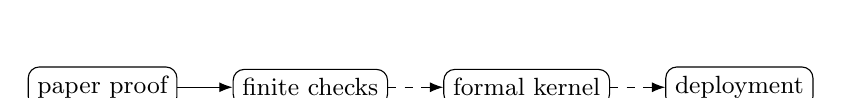
\begin{tikzpicture}[>=Latex,every node/.style={font=\small}]
\node[draw,rounded corners] (a) {paper proof};
\node[draw,rounded corners,right=0.7cm of a] (b) {finite checks};
\node[draw,rounded corners,right=0.7cm of b] (c) {formal kernel};
\node[draw,rounded corners,right=0.7cm of c] (d) {deployment};
\draw[->](a)--(b);\draw[->,dashed](b)--(c);\draw[->,dashed](c)--(d);
\end{tikzpicture}\caption{The final two verification transitions are unperformed obligations.}\end{figure}

\end{document}
